
\chapter{Results}
\label{cpt:results}

\section{Base Experiment}
\todo{Rewrite this section, it needs to be more readable. But the main content is here. When we compare algorithms we need to explain differences observed in terms of theoretical diferences between algorithms. Do the observed results concure with the expectation we have based on differences in implementations?}
\begin{figure}
    \centering
    \begin{subfigure}[b]{\textwidth}
            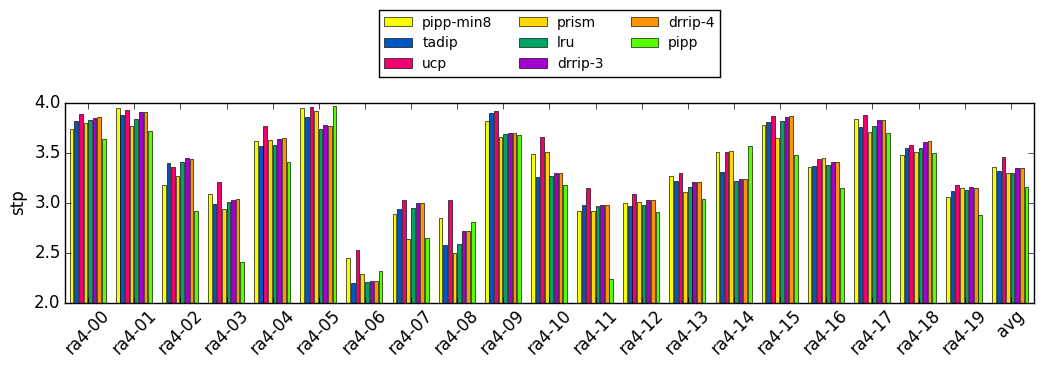
\includegraphics[width=\textwidth]{figures/results/speedup/stp-0128k-ra4}
            \caption{Random (ra4) workloads}
            \label{fig:results:4core:stp:random}
    \end{subfigure}

    \begin{subfigure}[b]{0.5\textwidth}
            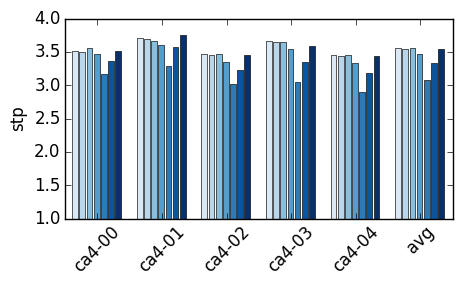
\includegraphics[width=\textwidth]{figures/results/speedup/stp-0128k-ca4}
            \caption{Cache (ca4) workloads}
            \label{fig:results:4core:stp:cache}
    \end{subfigure}%
    \begin{subfigure}[b]{0.5\textwidth}
            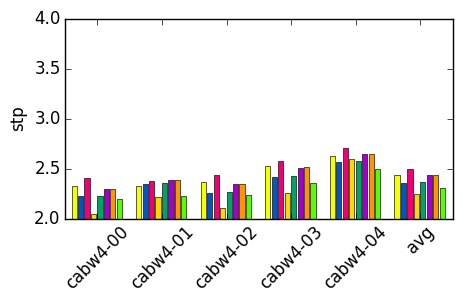
\includegraphics[width=\textwidth]{figures/results/speedup/stp-0128k-cabw4}
            \caption{Cache-Bandwidth (cabw4) workloads}
            \label{fig:results:4core:stp:cache-bw}
    \end{subfigure}

    \begin{subfigure}[b]{0.5\textwidth}
            \includegraphics[width=\textwidth]{figures/results/speedup/stp-0128k-bw4}
            \caption{Bandwidth (bw4) workloads}
            \label{fig:results:4core:stp:bw}
    \end{subfigure}%
    \begin{subfigure}[b]{0.5\textwidth}
            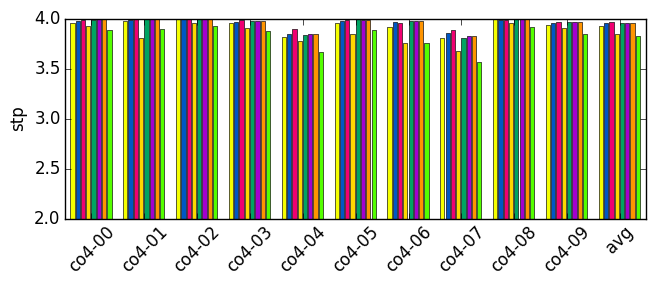
\includegraphics[width=\textwidth]{figures/results/speedup/stp-0128k-co4}
            \caption{Compute (co4) workloads}
            \label{fig:results:4core:stp:co}
    \end{subfigure}%

    \caption{4-Core workload STP results (128k L2)}\label{fig:results:4core:stp}
\end{figure}

\begin{figure}
    \centering
    \begin{subfigure}[b]{\textwidth}
            \includegraphics[width=\textwidth]{figures/results/speedup/hms-0128k-ra4}
            \caption{Random (ra4) workloads}
            \label{fig:results:4core:hms:random}
    \end{subfigure}

    \begin{subfigure}[b]{0.5\textwidth}
            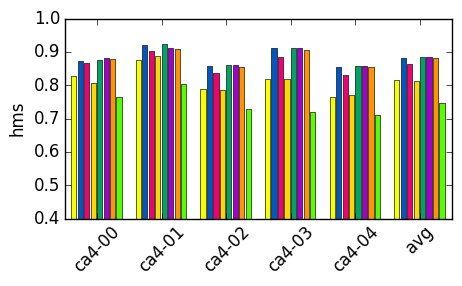
\includegraphics[width=\textwidth]{figures/results/speedup/hms-0128k-ca4}
            \caption{Cache (ca4) workloads}
            \label{fig:results:4core:hms:cache}
    \end{subfigure}%
    \begin{subfigure}[b]{0.5\textwidth}
            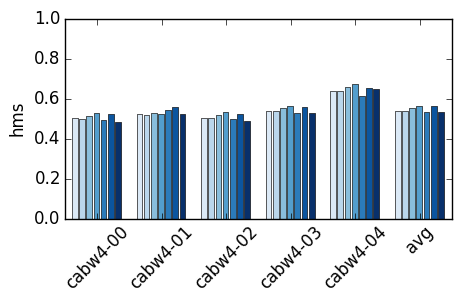
\includegraphics[width=\textwidth]{figures/results/speedup/hms-0128k-cabw4}
            \caption{Cache-Bandwidth (cabw4) workloads}
            \label{fig:results:4core:hms:cache-bw}
    \end{subfigure}

    \begin{subfigure}[b]{0.5\textwidth}
            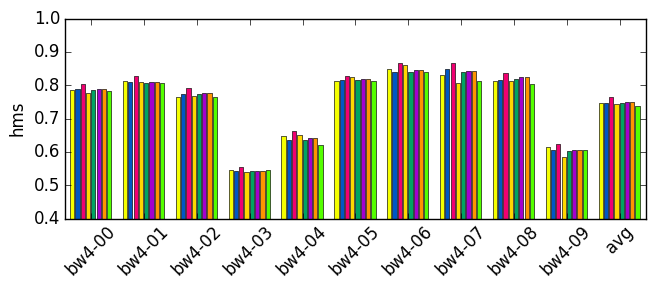
\includegraphics[width=\textwidth]{figures/results/speedup/hms-0128k-bw4}
            \caption{Bandwidth (bw4) workloads}
            \label{fig:results:4core:hms:bw}
    \end{subfigure}%
    \begin{subfigure}[b]{0.5\textwidth}
            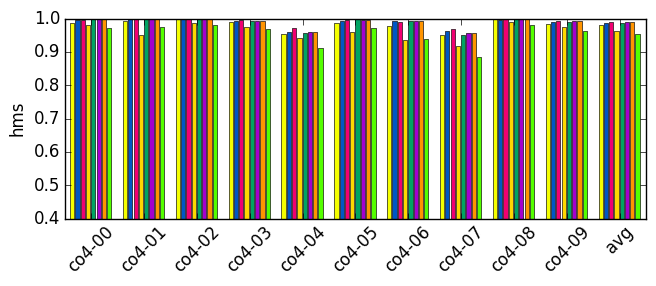
\includegraphics[width=\textwidth]{figures/results/speedup/hms-0128k-co4}
            \caption{Compute (co4) workloads}
            \label{fig:results:4core:hms:co}
    \end{subfigure}%

    \caption{4-Core workload HMS results (128k L2)}\label{fig:results:4core:hms}
\end{figure}

\begin{figure}
    \centering
    \begin{subfigure}[b]{\textwidth}
            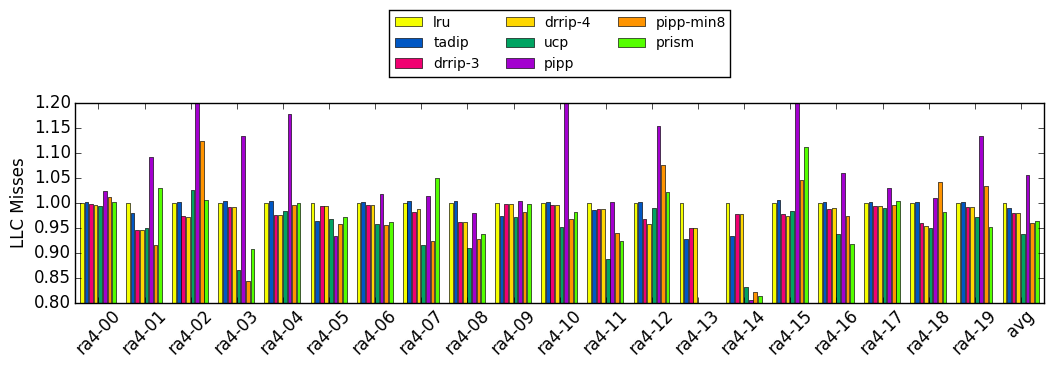
\includegraphics[width=\textwidth]{figures/results/misses/0128k-ra4}
            \caption{Random (ra4) workloads}
            \label{fig:results:4core:misses:random}
    \end{subfigure}

    \begin{subfigure}[b]{0.5\textwidth}
            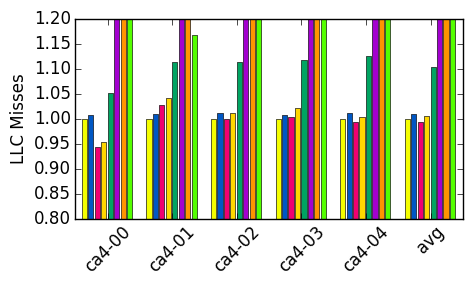
\includegraphics[width=\textwidth]{figures/results/misses/0128k-ca4}
            \caption{Cache (ca4) workloads}
            \label{fig:results:4core:misses:cache}
    \end{subfigure}%
    \begin{subfigure}[b]{0.5\textwidth}
            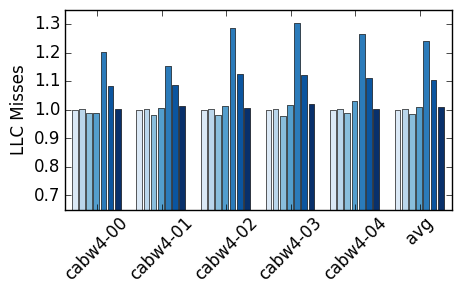
\includegraphics[width=\textwidth]{figures/results/misses/0128k-cabw4}
            \caption{Cache-Bandwidth (cabw4) workloads}
            \label{fig:results:4core:misses:cache-bw}
    \end{subfigure}

    \begin{subfigure}[b]{0.5\textwidth}
            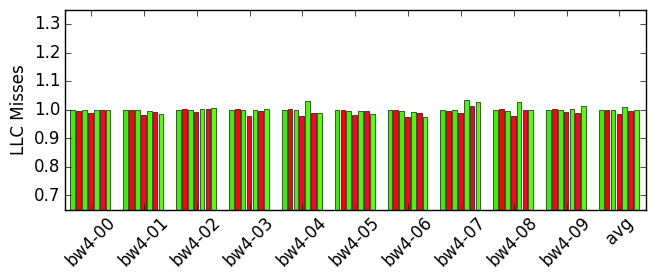
\includegraphics[width=\textwidth]{figures/results/misses/0128k-bw4}
            \caption{Bandwidth (bw4) workloads}
            \label{fig:results:4core:misses:bw}
    \end{subfigure}%
    \begin{subfigure}[b]{0.5\textwidth}
            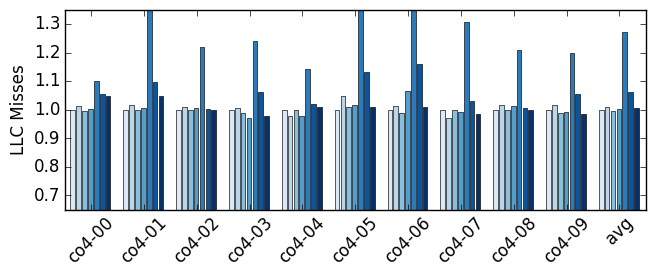
\includegraphics[width=\textwidth]{figures/results/misses/0128k-co4}
            \caption{Compute (co4) workloads}
            \label{fig:results:4core:misses:co}
    \end{subfigure}%

    \caption{4-Core workload LLC misses (128k L2)}\label{fig:results:4core:misses}
\end{figure}


\todo{This section is still a sketch, beware typos and incoherent reasoning}

For the cache bound 4-core workloads, we observe that LRU on average outperforms any other algorithm. 
PIPP on average performs worse, 15.7\% worse than LRU, with PIPP-min8 and PriSM just ahead at 8.4\% performance loss.
DRRIP performs on average as good as LRU. 
In the best case, ca4-00, DRRIP performs 1\% better than LRU.
In all other cases, all algorithms perform as good as or worse than LRU.
The result might be reasonable considering that these five workloads contain cache sensitive benchmarks, benchmarks whose performance is bounded by the available cache space, and which is not sensitive to changes in available bandwidth.
When running four benchmarks of this class in parallel we would expect them all to slow down, but they should not become memory bound.
Hence the slight changes in partition scheme should not have a big impact on either benchmark, and we should see negligible changes.
This is the case for three of the algorithms, TADIP, DRRIP and UCP.
For PIPP and PriSM, we observe a slowdown.
What the first three algorithms have in common is that they all will make use of the entire cache.
PIPP, on the other hand, inserts at lower positions and only misses can cause a block to move towards the MRU position.
Which four cache bound benchmarks we would expect PIPP to allocate about equal cache shared to each benchmark. \todo{We can rerun this workload with extended logging to see if this is the case}
As a result, PIPP may only insert in the lower quarter of the cache, and there is a chance only this part of the cache sees active usage.
If this is the case then forcing PIPP to insert higher should improve performance, which we observe as PIPP-min8 outperforms normal PIPP.
The PriSM algorithm also opens up to a reduced cache usage, and we see it perform as good as PIPP-min8.
The HMS results for this workload shows exactly the same trends.

For the bandwidth bound 4-core workloads we again see that one average all algorithms perform close to LRU.
Performance of bandwidth bound benchmarks is sensitive to available memory bandwidth, but not cache space. 
Due to this property we expect that no partition scheme will be able to improve performance, as the baseline performance is limited by excessive misses and little re-use.
The average speedup of bw4 workloads matches this expectation.
All algorithms except UCP performs within 0.1\% or LRU.
UCP has a noticeable performance gain of 2.6\%. 
This gain could be because UCP finds one benchmark in each workload with a small but exploitable reuse pattern and can take advantage of this by allocating most of the cache to this benchmark. \todo{Re-run this group with extended logging to see if this is the case, of so why does not PIPP also detect this? It might do, but due to the promotion policy it might just provide one hit, where UCP can provide multiple?}
\todo{Based on the extended logging results, can we link the gain to one or more benchmarks?}

Compute bounded, there should be nothing to gain. If the algorithm performs badly, i.e. causes more misses, it might decrease performance.
PIPP and PriSM slows down, significantly more misses, could again be because if the selected insert position. \todo{Run this PIPP on this group with extended logging, how does UMON allocate?}

In the Cache and bandwidth bound 4-core workloads, there is more room for performance gains. 
Benchmarks that are bound by both cache and bandwidth are most likely periodic, in that they sometimes are cache bound, and sometimes memory bound.
An example of this behavior would be a reduction step that handles much memory, and then a processing step that performs operations on the reduced data set.
A partitioning algorithm may be able to prioritize benchmarks that are currently cache sensitive.
DRRIP which is stream resistant given some conditions\todo{need to re-read the actual formulas and confirm if this property can be the cause of the speedup}  shows an average speedup of 2.9\% compared to LRU. 
This would indicate that DRRIP was able to reduce the amount of thrashing caused by benchmarks when they are bandwidth bound.
PIPP performs 2.8\% worse than LRU, but PIPP-min8 shows an equal speedup of 2.8\%. 
PIPP explicitly attempt to detect streaming applications and we therefore expected this algorithm to perform well in these conditions.
Examining the LCC miss rate we see that PIPP-min8, even thought it improves performance, it caused 9\% more misses than LRU.
These additional misses are most likely due to a few hits lost by streaming applications because PIPP inserted their row at or around LRU, compared to MRU under LRU replacement. 
\todo{Trivial to implement a logging that shows misses per core per state, i.e. l3.core0-miss-when-stream and l3.core0-miss-when-not-stream, could we use this to make a point here?}
The best performer in this group is UCP, which on average performs 5.5\% better than LRU.
The difference observed between PIPP and UCP is most likely due to the difference in promotion policy.
While both algorithms use the UMON with equal parameters to allocate cache rows, UCP promoted recency reuse while PIPP promotes base on reuse frequency. 
In these workloads, it would seem that the former is the optimal strategy.
While UCP does not explicitly detect streaming applications, we expect the UMON to allocate fewer rows to a streaming application because of the low reuse and hence utility. \todo{If we re-run these with extended logging we could plot average number of ways allocated to streaming cores, we would expect it to be about the same as the number of streaming cores.}
\todo{If the number of allocated ways is not close to one for all streaming cores, should the algorithm for PIPP be rewritten? Currently, we first allocate rows based on utility and then override if a core is streaming. However, if the streaming core was allocated say 16 rows, and we override it to 1, then there are 15 rows which are left unallocated. The PIPP paper is unclear on this, but if we find this to be the case we should probably rewrite the allocation for PIPP}

It could be argued that random workloads show a more real-world benchmark of the algorithms.
The average values show the same trend as the previous TADIP and DRRIP performs about equally to LRU.
PIPP is worse than LRU, but PIPP-min8 is an improvement.
Finally, UCP overall performs best.
In ra-13, we observe more than a 40\% decrease in LLC misses for PIPP-min8\todo{extend graph, bar not showing} giving a 3.2\% STP increase and a 20.7\% HMS increase.
However, TADIP at 1.8\% STP increase, and an HMS increase of 4.0\% shows a reduction of misses by less than 10\%.
This is a good demonstration of the fact that a reduction in misses does not directly translate to a proportional performance increase. 
ra-02 shows a increased LLC miss rate while also showing a performance improvement under PIPP-min8


8 and 16. We might have to redo these, as the available memory bandwidth was not scaled. Everything would have become bandwidth bounded.
\todo{We can especially see that PIPP and PIPP-min8, in general, increases the number of misses, as observed in the 4-core workloads, but, in general, this causes a loss and not a gain of performance here. 
If we scale the memory bandwidth, as we scale the LCC size, I believe PIPP will perform better.}


\todo{4-core with 512k L2 cache has been included; these will be evaluated in light of the above discussion. It might be interesting to plot total number of LLC accesses in the 512k case vs. the 128k case, as we expect a larger  L2 cache to filter out more of the LLC requests. One angle of the discussion would be to evaluate how a more filtered access pattern effect the algorithms.}



\begin{figure}
    \centering
    \begin{subfigure}[b]{\textwidth}
            \includegraphics[width=\textwidth]{figures/results/speedup/stp-0128k-ra8}
            \label{fig:results:4core:hms:random}
    \end{subfigure}

    \begin{subfigure}[b]{\textwidth}
            \includegraphics[width=\textwidth]{figures/results/speedup/hms-0128k-ra8}
            \label{fig:results:4core:hms:cache}
    \end{subfigure}
    \begin{subfigure}[b]{\textwidth}
            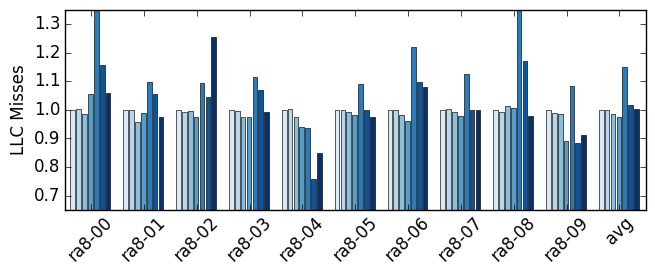
\includegraphics[width=\textwidth]{figures/results/misses/0128k-ra8}
            \label{fig:results:4core:hms:cache-bw}
    \end{subfigure}

    \caption{8-Core workload results (128k L2)}\label{fig:results:4core:hms}
\end{figure}

\begin{figure}
    \centering
    \begin{subfigure}[b]{\textwidth}
            \includegraphics[width=\textwidth]{figures/results/speedup/stp-0128k-ra16}
            \label{fig:results:4core:hms:random}
    \end{subfigure}

    \begin{subfigure}[b]{\textwidth}
            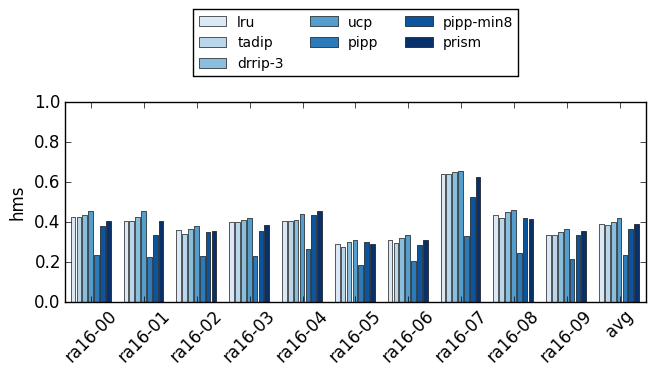
\includegraphics[width=\textwidth]{figures/results/speedup/hms-0128k-ra16}
            \label{fig:results:4core:hms:cache}
    \end{subfigure}
    \begin{subfigure}[b]{\textwidth}
            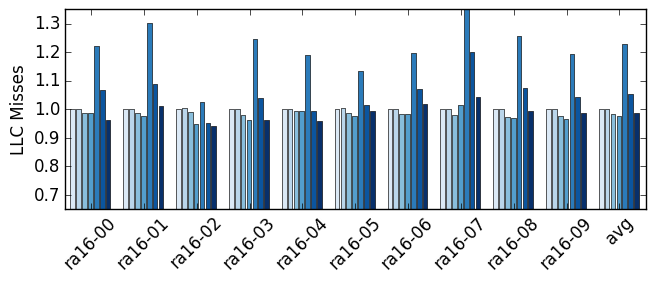
\includegraphics[width=\textwidth]{figures/results/misses/0128k-ra16}
            \label{fig:results:4core:hms:cache-bw}
    \end{subfigure}

    \caption{16-Core workload results (128k L2)}\label{fig:results:4core:hms}
\end{figure}


\section{L2 Sensitivity}

\todo{This section should cover results from varying L2 size. It is probably not a good idea to have all graphs for all runs, we should find a way to aggregate while keeping all important details.}

\begin{figure}
    \centering
    \begin{subfigure}[b]{\textwidth}
            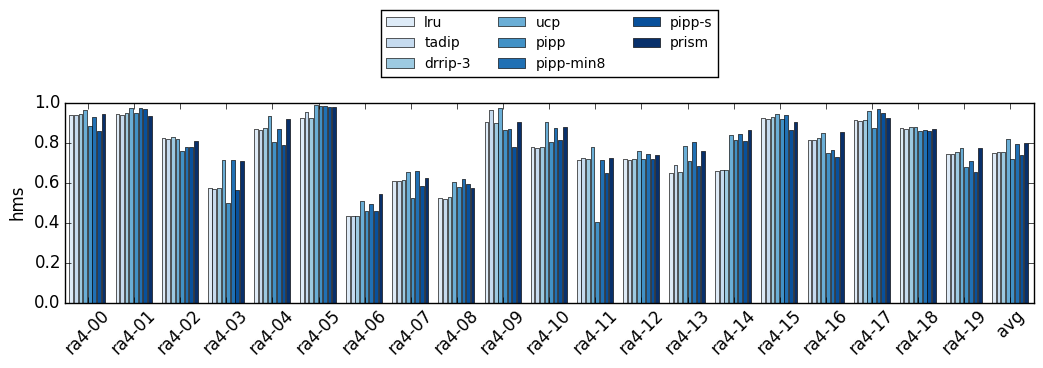
\includegraphics[width=\textwidth]{figures/results/speedup/hms-0512k-ra4}
            \caption{Random (ra4) workloads}
            \label{fig:results:4core:hms:random}
    \end{subfigure}

    \begin{subfigure}[b]{0.5\textwidth}
            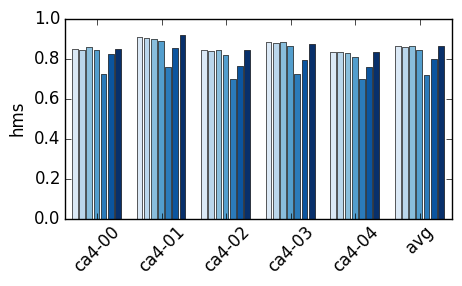
\includegraphics[width=\textwidth]{figures/results/speedup/hms-0512k-ca4}
            \caption{Cache (ca4) workloads}
            \label{fig:results:4core:hms:cache}
    \end{subfigure}%
    \begin{subfigure}[b]{0.5\textwidth}
            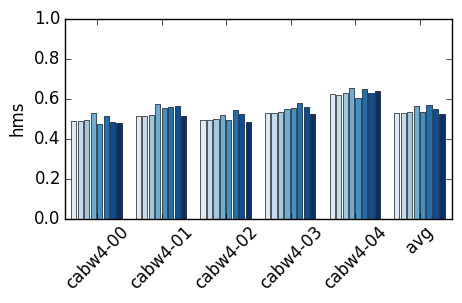
\includegraphics[width=\textwidth]{figures/results/speedup/hms-0512k-cabw4}
            \caption{Cache-Bandwidth (cabw4) workloads}
            \label{fig:results:4core:hms:cache-bw}
    \end{subfigure}

    \begin{subfigure}[b]{0.5\textwidth}
            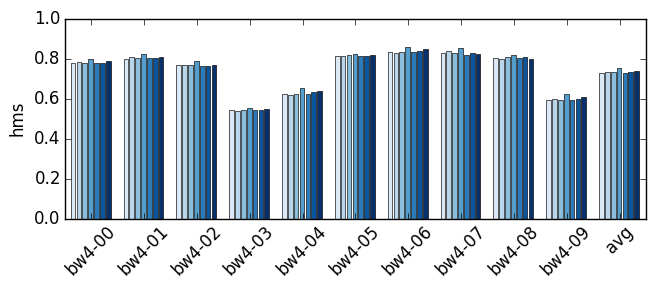
\includegraphics[width=\textwidth]{figures/results/speedup/hms-0512k-bw4}
            \caption{Bandwidth (bw4) workloads}
            \label{fig:results:4core:hms:bw}
    \end{subfigure}%
    \begin{subfigure}[b]{0.5\textwidth}
            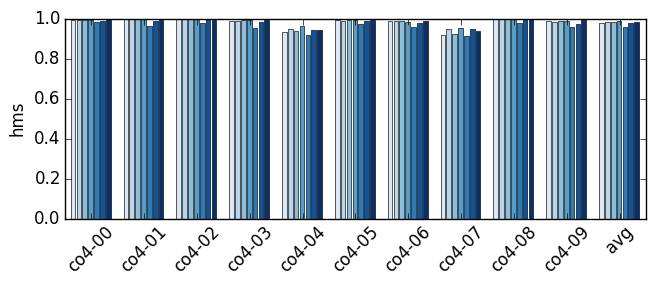
\includegraphics[width=\textwidth]{figures/results/speedup/hms-0512k-co4}
            \caption{Compute (co4) workloads}
            \label{fig:results:4core:hms:co}
    \end{subfigure}%

    \caption{4-Core workload HMS results (512k L2)}\label{fig:results:4core:hms}
\end{figure}

\begin{figure}
    \centering
    \begin{subfigure}[b]{\textwidth}
            \includegraphics[width=\textwidth]{figures/results/misses/0512k-ra4}
            \caption{Random (ra4) workloads}
            \label{fig:results:4core:misses:random}
    \end{subfigure}

    \begin{subfigure}[b]{0.5\textwidth}
            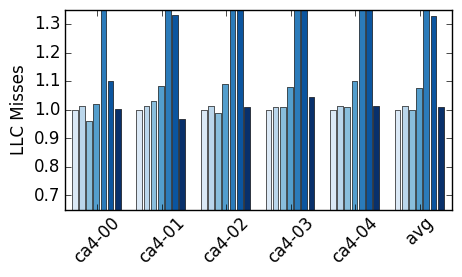
\includegraphics[width=\textwidth]{figures/results/misses/0512k-ca4}
            \caption{Cache (ca4) workloads}
            \label{fig:results:4core:misses:cache}
    \end{subfigure}%
    \begin{subfigure}[b]{0.5\textwidth}
            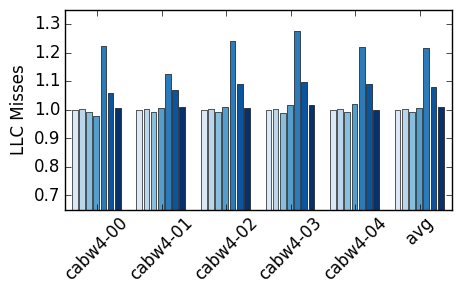
\includegraphics[width=\textwidth]{figures/results/misses/0512k-cabw4}
            \caption{Cache-Bandwidth (cabw4) workloads}
            \label{fig:results:4core:misses:cache-bw}
    \end{subfigure}

    \begin{subfigure}[b]{0.5\textwidth}
            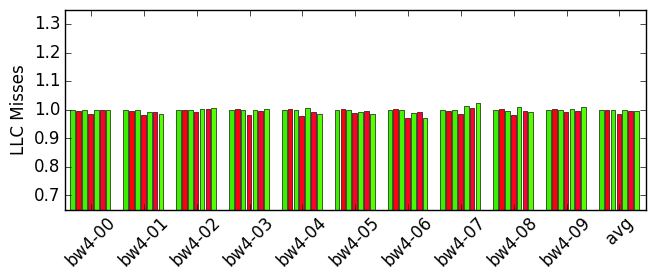
\includegraphics[width=\textwidth]{figures/results/misses/0512k-bw4}
            \caption{Bandwidth (bw4) workloads}
            \label{fig:results:4core:misses:bw}
    \end{subfigure}%
    \begin{subfigure}[b]{0.5\textwidth}
            \includegraphics[width=\textwidth]{figures/results/misses/0512k-co4}
            \caption{Compute (co4) workloads}
            \label{fig:results:4core:misses:co}
    \end{subfigure}%

    \caption{4-Core workload LLC misses (512k L2)}\label{fig:results:4core:misses}
\end{figure}



\begin{figure}
    \centering
    \begin{subfigure}[b]{\textwidth}
            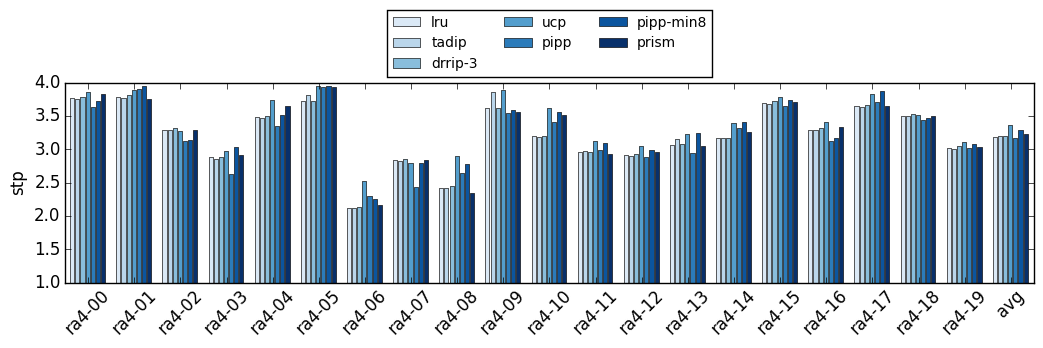
\includegraphics[width=\textwidth]{figures/results/speedup/stp-0512k-ra4}
            \caption{Random (ra4) workloads}
            \label{fig:results:4core:stp:random}
    \end{subfigure}

    \begin{subfigure}[b]{0.5\textwidth}
            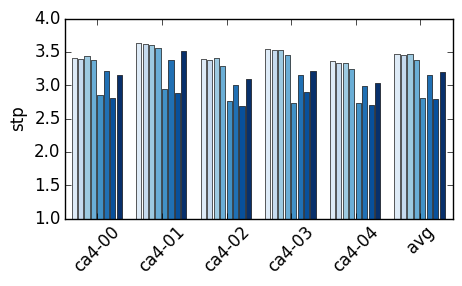
\includegraphics[width=\textwidth]{figures/results/speedup/stp-0512k-ca4}
            \caption{Cache (ca4) workloads}
            \label{fig:results:4core:stp:cache}
    \end{subfigure}%
    \begin{subfigure}[b]{0.5\textwidth}
            \includegraphics[width=\textwidth]{figures/results/speedup/stp-0512k-cabw4}
            \caption{Cache-Bandwidth (cabw4) workloads}
            \label{fig:results:4core:stp:cache-bw}
    \end{subfigure}

    \begin{subfigure}[b]{0.5\textwidth}
            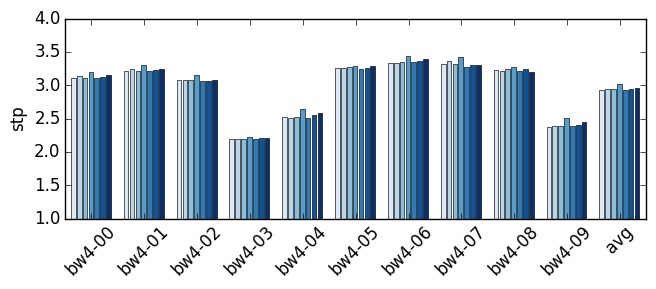
\includegraphics[width=\textwidth]{figures/results/speedup/stp-0512k-bw4}
            \caption{Bandwidth (bw4) workloads}
            \label{fig:results:4core:stp:bw}
    \end{subfigure}%
    \begin{subfigure}[b]{0.5\textwidth}
            \includegraphics[width=\textwidth]{figures/results/speedup/stp-0512k-co4}
            \caption{Compute (co4) workloads}
            \label{fig:results:4core:stp:co}
    \end{subfigure}%

    \caption{4-Core workload STP results (512k L2)}\label{fig:results:4core:stp}
\end{figure}

\section{Simulator Parallelism Sentitivity}
\todo{As above, but along a different axis}